\chapter{Inserting objects}
\ifpdf
  \graphicspath{{Chapter2/Chapter2Figs/}}
\else
\graphicspath{{Chapter2/Chapter2Figs/EPS/}{Chapter2/Chapter2Figs/}}
\fi

%
Hand-drawn figures, downloaded/created images \& graphs need to be inserted in a document. There are different ways to insert these in a document. 


\section{Insert an image}

One image as in Figure \ref{Fig21} is to be inserted. Looks good if it is located in the center. The size can be adjusted to suit the needs. 

\begin{figure}[!htbp]
  \begin{center}
    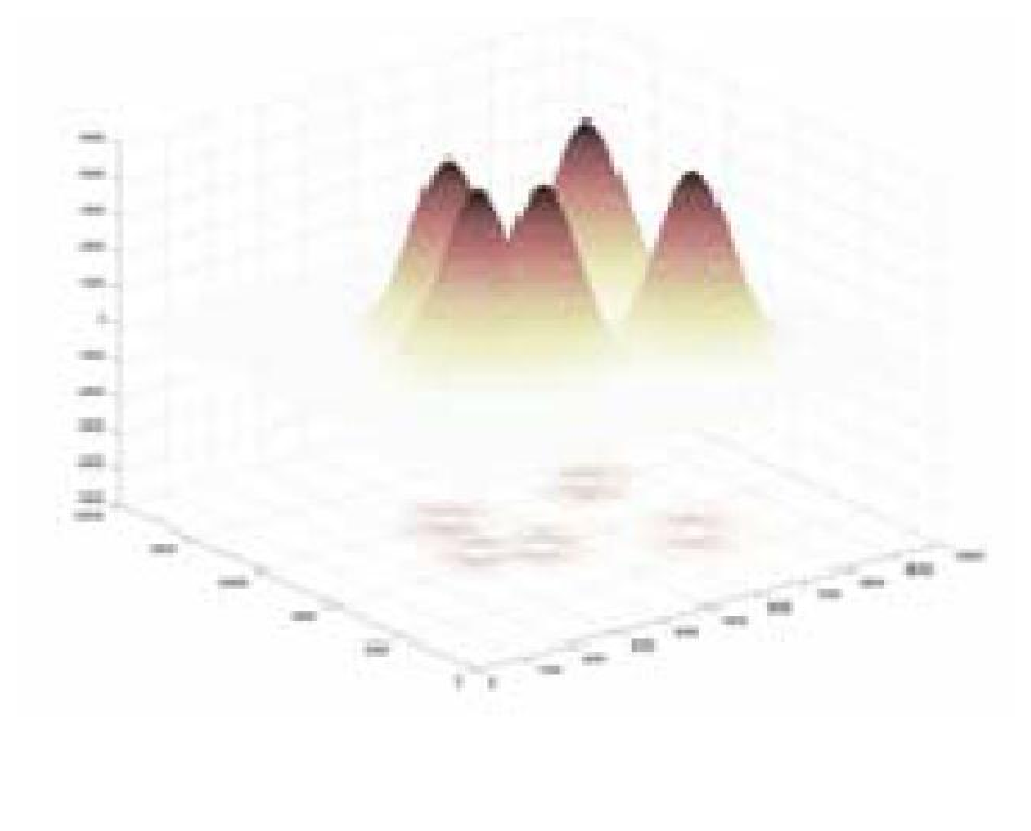
\includegraphics [scale=0.5]{small_width}
    \caption{Gaussian kernel}
    \label{Fig21}
  \end{center}
\end{figure}

\section{Insert a graph}

 Graph could be included as any other image or figure. Figure \ref{Fig24} shows a single plot. \\ 

\begin{figure}[!htbp]
  \begin{center}
    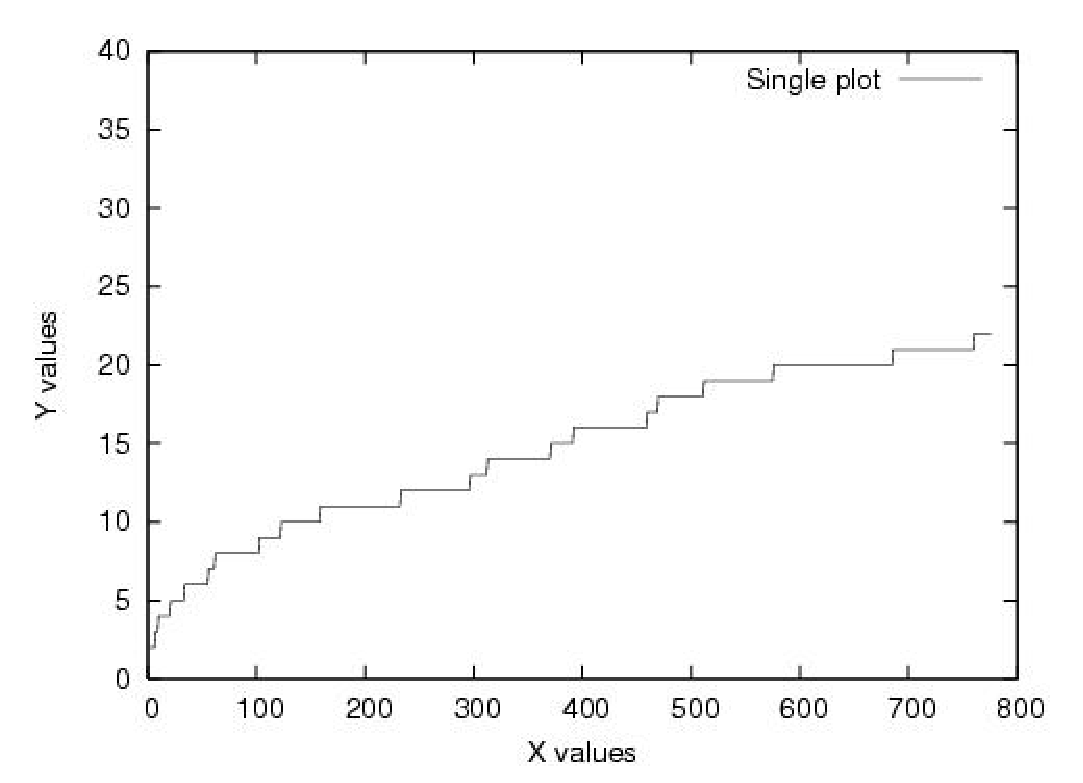
\includegraphics [scale=0.5]{single_plot}
    \caption{Single plot on a graph}
    \label{Fig24}
  \end{center}
\end{figure}

%------------------------------------------------------------------------
